% Intended LaTeX compiler: pdflatex
\documentclass[koma,a4paper,utopia,12pt,listings-color,microtype,paralist,colorlinks,urlcolor=red]{org-article}
       \usepackage{tikz}
       \usetikzlibrary{arrows,decorations.pathmorphing}
       \usetikzlibrary{backgrounds,positioning,fit,petri}
               \usepackage{tikz}
\author{Eason}
\date{\today}
\title{Walk Through the Petri-Net In TiKZ Tutorial}
\hypersetup{
 pdfauthor={Eason},
 pdftitle={Walk Through the Petri-Net In TiKZ Tutorial},
 pdfkeywords={},
 pdfsubject={Analyze the Petri-Net tutorial in Chapter 3 of the TikZ manual line by line.},
 pdfcreator={Emacs 26.3 (Org mode 9.2.6)},
 pdflang={English}}
\begin{document}




 \thispagestyle{empty}
 \begingroup
\begin{center}
 \vspace{\baselineskip}
 \textbf{\Huge Walk Through the Petri-Net In TiKZ Tutorial} \par
 \vspace{2\baselineskip}  \newline
 \textbf{\large Eason Zhang with www.makesteamclear.com \par}
 \vspace{\baselineskip} \newline
  \today \par
 \vspace{\baselineskip}
  \vfill
 \setlength{\unitlength}{3pt}
 \includegraphics[width=0.5\textwidth]{/Users/chaolongzhang/Dropbox/mstemc_hugo/static/img/tikz/petrinetfinal.pdf}
 \vfill \vspace{\baselineskip}
 \href{WWW.MAKESTEAMCLEAR.COM}{\Large WWW.MAKESTEAMCLEAR.COM} \par\newline
  makesteamclear is a free project, run by Eason Zhang, to make videos about STEAM in a more approachable way. If you find the contents in this article or the site or the youtube channel helpful, please consider \href{www.makesteamclear.com}{\ensuremath \heartsuit support me\ensuremath\heartsuit }, thanks \par
 \end{center}
 \endgroup

 \newpage \thispagestyle{empty} \textbf{copyright page} \newpage \tableofcontents \newpage
\hspace{0pt}\\

Analyze the Petri-Net tutorial in Chapter 3 of the TikZ manual line by line.

Chapter 3 of the TikZ tutorial gives an example of Petri net. In this post, let
me work through the code line by line. During this example, more tikz libraries
are used, such as \texttt{arrows} , \texttt{decorations.pathmorphing} , \texttt{backgrounds} ,
\texttt{positioning} , \texttt{fit}, \texttt{petri} . These libraries should be added before the
\texttt{tikzpicture} environment.

\begin{center}
\includegraphics[width=0.8\textwidth]{/Users/chaolongzhang/Dropbox/mstemc_hugo/static/img/tikz/petrinet.pdf}
\end{center}

The code is shown as
\lstset{language=[LaTeX]TeX,label= ,caption= ,captionpos=b,firstnumber=1,numbers=left}
\begin{lstlisting}
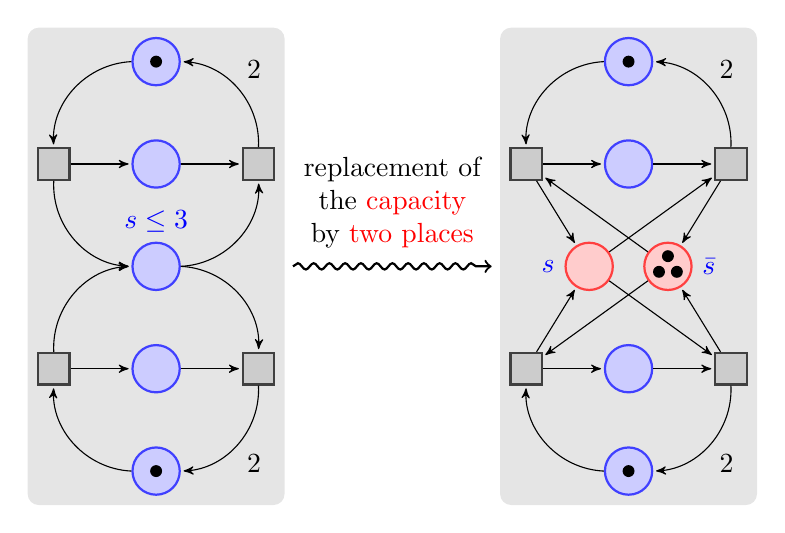
\begin{tikzpicture}
  [node distance=1.3cm,on grid,>=stealth',bend angle=45,auto,
  every place/.style= {minimum size=6mm,thick,draw=blue!75,fill=blue!20},
  every transition/.style={thick,draw=black!75,fill=black!20},
  red place/.style= {place,draw=red!75,fill=red!20},
  every label/.style= {blue}]
  \node [place,tokens=1] (w1) {};
  \node [place] (c1) [below=of w1] {};
  \node [place] (s) [below=of c1,label=above:$s\le 3$] {};
  \node [place] (c2) [below=of s] {};
  \node [place,tokens=1] (w2) [below=of c2] {};
  \node [transition] (e1) [left=of c1] {}
  edge [pre,bend left] (w1)
  edge [post,bend right] (s)
  edge [post] (c1);
  \node [transition] (e2) [left=of c2] {}
  edge [pre,bend right] (w2)
  edge [post,bend left] (s)
  edge [post] (c2);
  \node [transition] (l1) [right=of c1] {}
  edge [pre] (c1)
  edge [pre,bend left] (s)
  edge [post,bend right] node[swap] {2} (w1);
  \node [transition] (l2) [right=of c2] {}
  edge [pre] (c2)
  edge [pre,bend right] (s)
  edge [post,bend left] node {2} (w2);

  \begin{scope}[xshift=6cm]
    \node [place,tokens=1] (w1') {};
    \node [place] (c1') [below=of w1'] {};
    \node [red place] (s1') [below=of c1',xshift=-5mm]
    [label=left:$s$] {};
    \node [red place,tokens=3] (s2') [below=of c1',xshift=5mm]
    [label=right:$\bar s$] {};
    \node [place] (c2') [below=of s1',xshift=5mm] {};
    \node [place,tokens=1] (w2') [below=of c2'] {};
    \node [transition] (e1') [left=of c1'] {}
    edge [pre,bend left] (w1')
    edge [post] (s1')
    edge [pre] (s2')
    edge [post] (c1');
    \node [transition] (e2') [left=of c2'] {}
    edge [pre,bend right] (w2')
    edge [post] (s1')
    edge [pre] (s2')
    edge [post] (c2');
    \node [transition] (l1') [right=of c1'] {}
    edge [pre] (c1')
    edge [pre] (s1')
    edge [post] (s2')
    edge [post,bend right] node[swap] {2} (w1');
    \node [transition] (l2') [right=of c2'] {}
    edge [pre] (c2')
    edge [pre] (s1')
    edge [post] (s2')
    edge [post,bend left] node {2} (w2');
  \end{scope}
  \begin{scope}[on background layer]
    \node (r1) [fill=black!10,rounded corners,fit=(w1)(w2)(e1)(e2)(l1)(l2)] {};
    \node (r2) [fill=black!10,rounded corners,fit=(w1')(w2')(e1')(e2')(l1')(l2')] {};
  \end{scope}
  \draw [shorten >=1mm,-to,thick,decorate,
  decoration={snake,amplitude=.4mm,segment length=2mm,
    pre=moveto,pre length=1mm,post length=2mm}]
  (r1) -- (r2) node [above=1mm,midway,text width=3cm,align=center]
  {replacement of the \textcolor{red}{capacity} by \textcolor{red}{two places}};
\end{tikzpicture}
\end{lstlisting}
\end{document}
